\subsection{Design Constraints}

\subsubsection{Software Constraints}
\begin{enumerate}
	\item Device Accelerometer Support:
	\newline
	Given that a device does has an accelerometer, the device manufacturer must provide a software interface to interact with the device's accelerometer.
\end{enumerate}

\subsubsection{Hardware Constraints}
\begin{enumerate}
	\item Accelerometer:
	\newline
	Not all devices models are made equal. Some older devices do not have accelerometers to track steps with. The accuracy of accelerometers also vary from different device manufacturers.
	\item Battery Life:
	\newline
	To track steps continuously with a background process will greatly impact the battery life of devices with small battery capacities. 
\end{enumerate}

\subsection{Activity Diagram}
See figure~\ref{fig:fitness_activity_diagram} on page~\pageref{fig:fitness_activity_diagram}
\begin{figure}
	\centering
	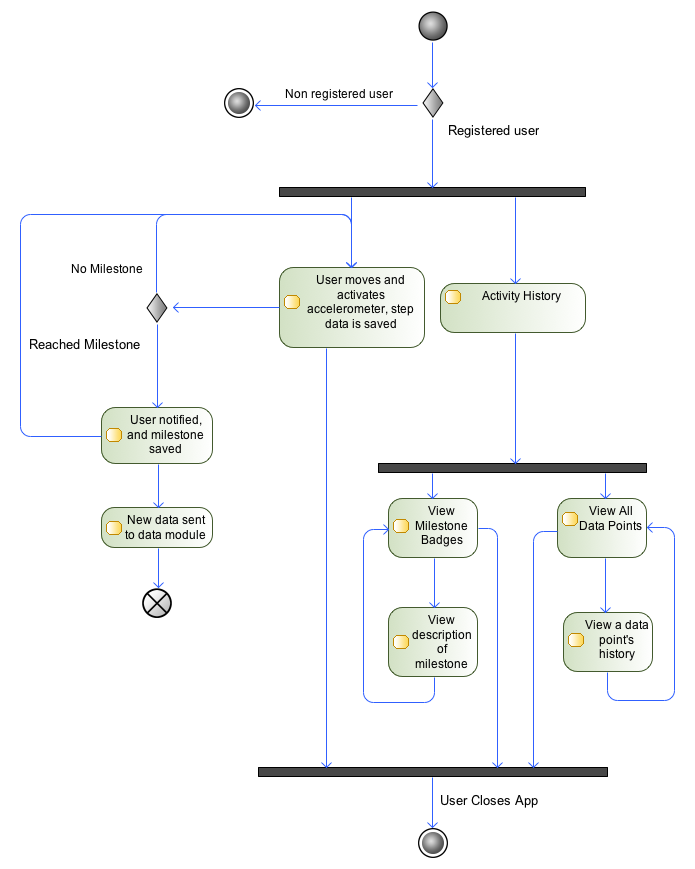
\includegraphics[scale=0.54]{Fitness/fitness_activity_diagram.png}
	\caption{Fitness Activity Diagram}
	\label{fig:fitness_activity_diagram}
\end{figure}

\subsection{State Diagrams}
See figure~\ref{fig:fitness_state_diagram} on page~\pageref{fig:fitness_state_diagram}
\begin{figure}
	\centering
	\includegraphics[scale=0.54]{Fitness/fitness_state_diagram.png}
	\caption{Fitness State Diagram}
	\label{fig:fitness_state_diagram}
\end{figure}

\subsection{Deployment Diagram}
See figure~\ref{fig:fitness_deployment_diagram} on page~\pageref{fig:fitness_deployment_diagram}
\begin{figure}
	\centering
	\includegraphics[scale=0.54]{Fitness/fitness_deployment_diagram.png}
	\caption{Fitness Deployment Diagram}
	\label{fig:fitness_deployment_diagram}
\end{figure}